\section{Оптимизация}
\label{sec:Optimization}

Оптимизацией должен являться LLVM Pass из LLVM IR в LLVM IR в векторном
backend'е графического компилятора Intel. Для упрощения проектирования,
реализации и поддержки, оптимизация разделена на две части: анализ и
трансформацию.

Перед рассмотрением анализа и трансформации, проведем обзор возможных
конструкций, которые ожидаются на вход оптимизации.

Так как рассматривается только структурированный поток управления, то можно
рассматривать только два атомарных случая: векторный условный переход и
векторный цикл. На рисунках ~\ref{fig:if-else-simdcf-simple} и
~\ref{fig:loop-simdcf-simple} представлен граф потока управления для if-else и
цикла соответственно.
\begin{figure}
  \centering
  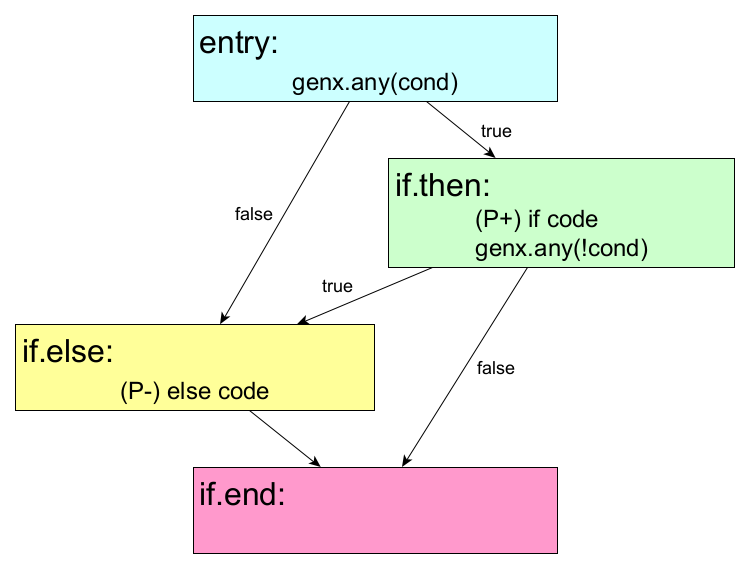
\includegraphics[scale=0.27]{Images/if-else-FE-colored.png}
  \caption{Схема потока управления для if-else}
  \label{fig:if-else-simdcf-simple}
\end{figure}
\begin{figure}
  \centering
  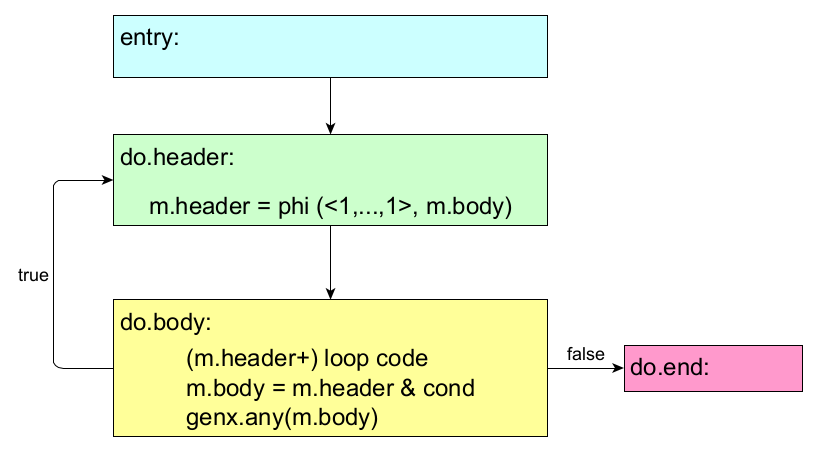
\includegraphics[scale=0.27]{Images/do-while-FE-colored.png}
  \caption{Схема потока управления для цикла}
  \label{fig:loop-simdcf-simple}
\end{figure}

В реальном коде может встречаться сложный поток управления, в котором базовые
паттерны могут являться элементами других базовых паттернов, образовывая
вложенные конструкции, например if-else вложенный в if-else (рисунок
~\ref{fig:nested-if-simdcf}) или цикл с вложенным if-else (рисунок
~\ref{fig:loop-nested-if-simdcf}).
\begin{figure}
  \centering
  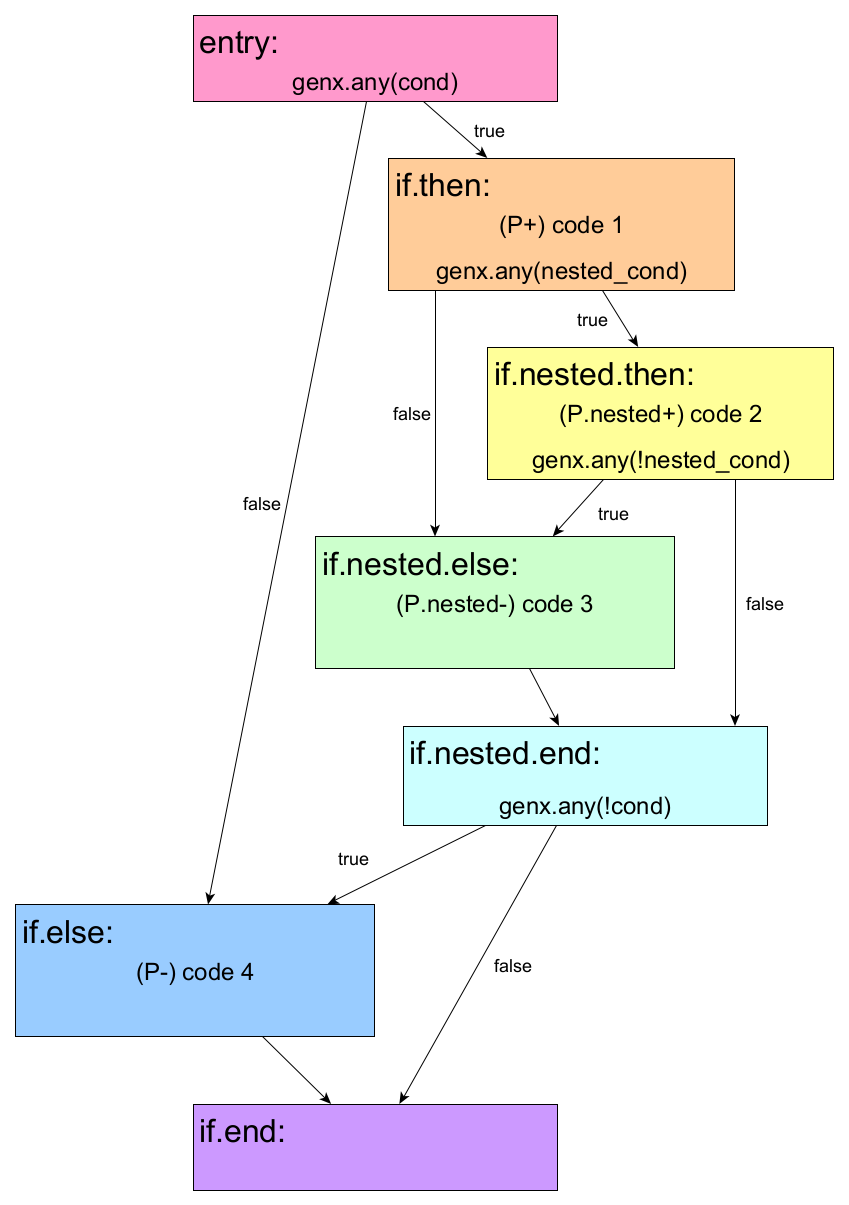
\includegraphics[scale=0.27]{Images/nested-if-FE-colored.png}
  \caption{Схема потока управления для случая if-else вложенного в if-else}
  \label{fig:nested-if-simdcf}
\end{figure}
\begin{figure}
  \centering
  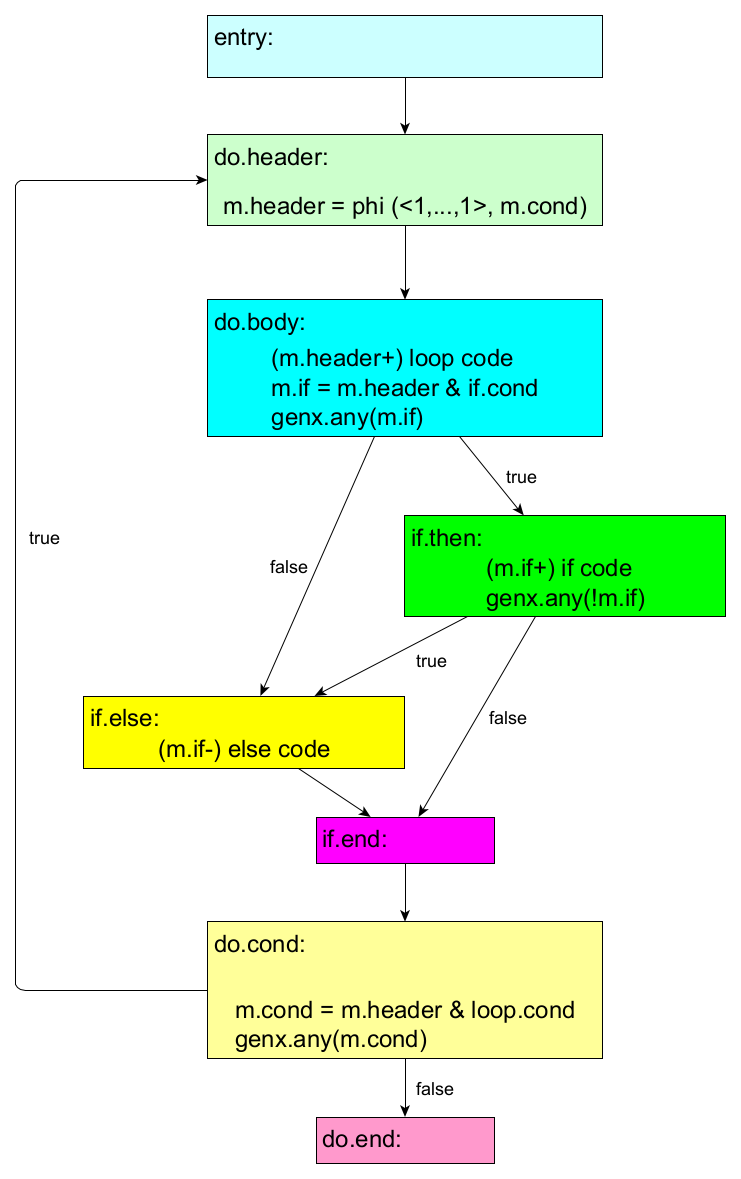
\includegraphics[scale=0.27]{Images/do-while-nested-if-FE-colored.png}
  \caption{Схема потока управления для случая if-else вложенного в цикл}
  \label{fig:loop-nested-if-simdcf}
\end{figure}

Можно выделить регионы, содержащие в себе одну конструкцию векторного потока
управления определенного уровня вложенности. Определим SIMD CF регион как
регион, содержащий в себе одну конструкцию предложенного ранее интерфейса самого
внешнего уровня вложенности, доступного для данного региона. Такой подход
позволит упростить анализ, позволяя сначала обнаруживать самые внешние SIMD CF
регионы, а после - вложенные. Тогда обобщенные SIMD CF регионы будут выглядеть
как на рисунках ~\ref{fig:generalized-if-simdcf} и ~\ref{fig:generalized-loop-simdcf}.
\begin{figure}
  \centering
  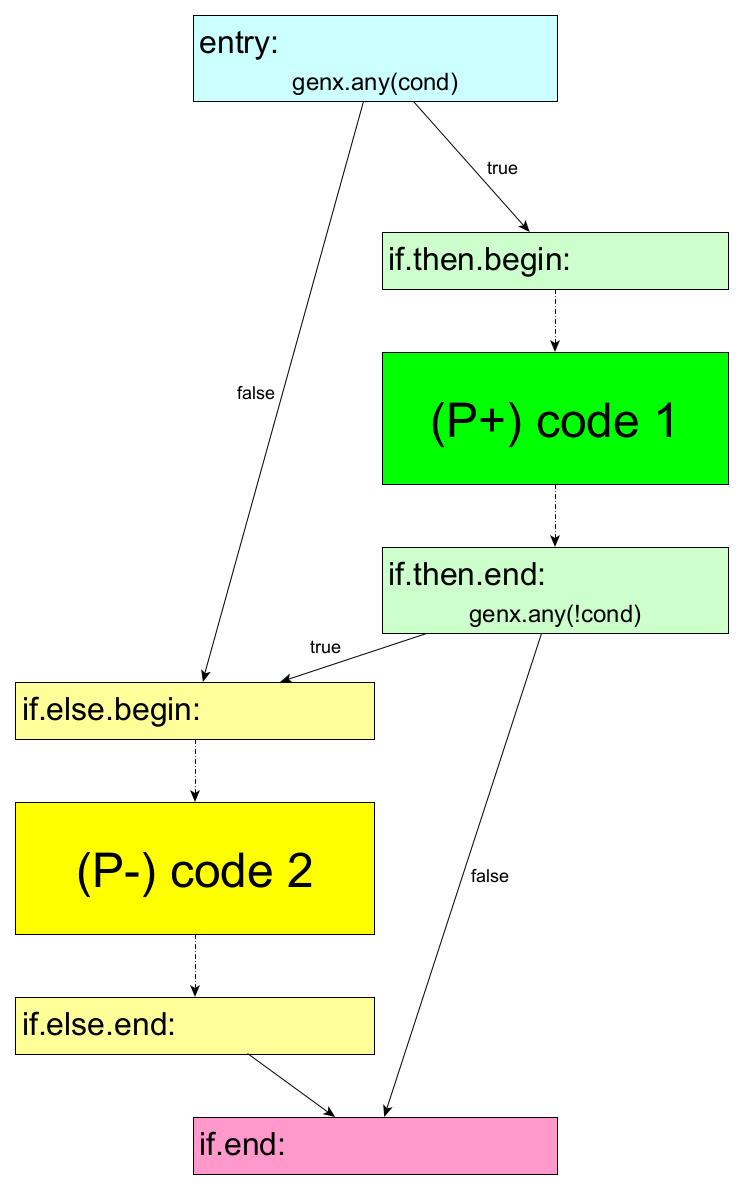
\includegraphics[scale=0.27]{Images/if-else-FE-generalized-colored.png}
  \caption{Схема if-else SIMD CF региона}
  \label{fig:generalized-if-simdcf}
\end{figure}
\begin{figure}
  \centering
  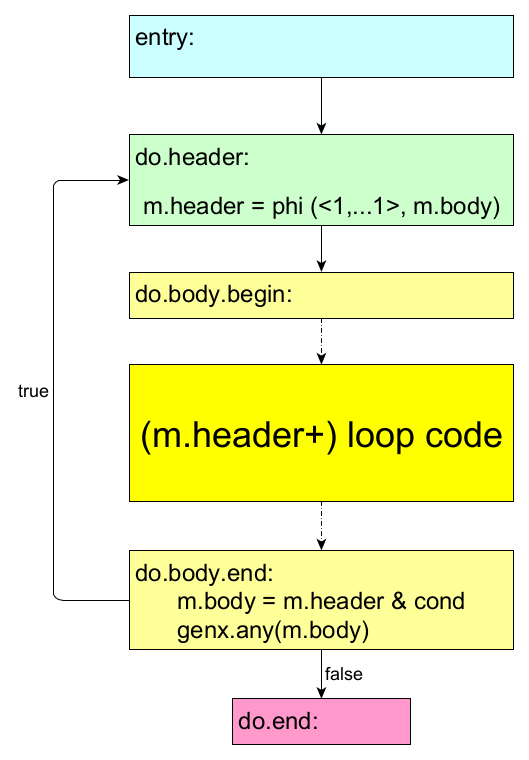
\includegraphics[scale=0.27]{Images/do-while-FE-generalized-colored.png}
  \caption{Схема if-else SIMD CF региона}
  \label{fig:generalized-loop-simdcf}
\end{figure}

После определения SIMD CF региона можно свести задачу поиска заранее оговоренных
конструкций к поиску SIMD CF регионов самого внешнего уровня вложенности, после
чего искать вложенные SIMD CF регионы.

Шаг 1. Поиск условного перехода, похожего на векторный поток управления. Для
каждого базового блока проверяется его терминатор. Если это инструкция условного
перехода, то проверяется его условие, в противном случае конструкция не является
SIMD CF регионом. Если условием является результат вызова одного из обозначенных
ранее интринсиков, то идет переход к шагу 2.

Шаг 2. Проверяется структура потока управления и происходит попытка сопоставить
его либо с SIMD CF if/else, либо с SIMD CF циклом. Если сопоставление с одним из
заданных паттернов невозможно, то конструкция не является SIMD CF регионом. В
противном случае происходит переход к шагу 3.

Шаг 3. Проверка маскирования побочных эффектов. Для каждой инструкции, у которой
есть побочные эффекты проводится проверка, является ли такая инструкция
маскирована и если она маскирована, то проверяется, совпадает ли маска для
данной инструкции с условием перехода в эту дугу. Для вложенных регионов
проверяется, является ли маска данного региона подмножеством маски внешнего
региона. Если проверка неудачная - данный регион не является SIMD CF регионом.

Дополнение к шагу 3 для цикла. Проверяются фи-узлы для индуктивностей и пересчет
маски для каждого цикла. Если проверка неудачная - данный регион не является
SIMD CF регионом. В противном случае идет переход к шагу 4.

Дополнение к шагу 3 для if-else. Если кроме if также имеется else, то происходит
проверка, являются ли маски if и else строго противоположны друг другу. Если
проверка неудачная - данный регион не является SIMD CF регионом. В противном
случае идет переход к шагу 4.

Шаг 4. Данный регион является SIMD CF регионом. Аналогично происходит поиск
вложенных SIMD CF регионов для данного региона.

В псевдокоде данный алгоритм будет выглядеть следующим образом:

\begin{verbatim}
procedure Find_SIMD_CF_Regions(Reg) returns set of SIMD_CF_Region
  Reg: Region
begin
  regions: set of SIMD_CF_Region
  bb: Basic_Block
  for each bb ∈ Reg do
    if Is_SIMD_CF_Branch(bb.terminator) then
      match: SIMD_CF_Region
      match := Match(bb)
      if match then
        if Verify(match) then
          regions ⋃= match
        fi
      fi
    fi
  od
  return regions
end

procedure Is_SIMD_CF_Branch(Term) return boolean
  Term: Instruction
begin
  cond: Instruction
  cond := Term.condition
  return cond ∈ {llvm.vector.reduce.and, llvm.vector.reduce.or}
end

procedure Match(BB) return SIMD_CF_Region
  BB: Basic_Block
begin
  if MatchIf(BB) then
    return SIMD_CF_If_Region(BB)
  elif MatchLoop(BB) then
    return SIMD_CF_Loop_Region(BB)
  else
    return nil
end

procedure MatchIf(Entry) return SIMD_CF_If_Region
  Entry: Basic_Block
begin
  subregions: set of SIMD_CF_Region
  has_else: boolean
  if_begin: Basic_Block
  if_end: Basic_Block
  else_begin: Basic_Block
  else_end: Basic_Block
  exit: Basic_Block
  if_begin := Entry.true_succ
  else_begin := Entry.false_succ
  pred: Basic_Block
  for each pred ∈ else_begin.preds do
    if pred ≠ Entry then
      if_end := pred
    fi
  od
  subregions ⋃= Find_SIMD_CF_Regions(Region(if_begin, if_end))
  if !if_end.terminator.conditional then
    has_else := false
    exit := else_begin
    return SIMD_CF_If_Region(Entry, exit, has_else, subregions)
  fi
  has_else := true
  exit := if_end.false_succ
  for each pred ∈ exit.preds do
    if pred ≠ if_end then
      else_end := pred
    fi
  od
  subregions ⋃= Find_SIMD_CF_Regions(Region(else_begin, else_end))
  return SIMD_CF_If_Region(Entry, exit, has_else, subregions)
end

procedure MatchLoop(BranchingBB) return SIMD_CF_Loop_Region
  BranchingBB: Basic_Block
begin
  loop: Loop
  loop := Get_Loop(BranchingBB)
  if !loop then
    return nil
  fi
  subregions ⋃= Find_SIMD_CF_Regions(Region(loop.entering, loop.exiting))
  return SIMD_CF_Loop_Region(loop, subregions)
end

procedure Verify(R) return boolean
  R: SIMD_CF_Region
begin
  inst: Instruction
  subreg: SIMD_CF_Region
  for each inst ∈ R do
    if inst.has_side_effects then
      if inst.mask ≠ R.mask then
        return false
      fi
    fi
  od
  for each subreg ∈ R.subregions do
    if !R.is_submask(subreg_mask) then
      return false
    fi
  od
  return true
end
\end{verbatim}

После сбора всей информации о SIMD CF регионах начинается их оптимизирующая
трансформация.

Для этого сначала рассмотрим текущую модель \texttt{goto}-\texttt{join} в
векторном backend'е графического компилятора Intel. Текущая модель для условных
переходов и циклов показана на рисунках ~\ref{fig:if-goto-join-BE} и
~\ref{fig:loop-goto-join-BE}.
\begin{figure}
  \centering
  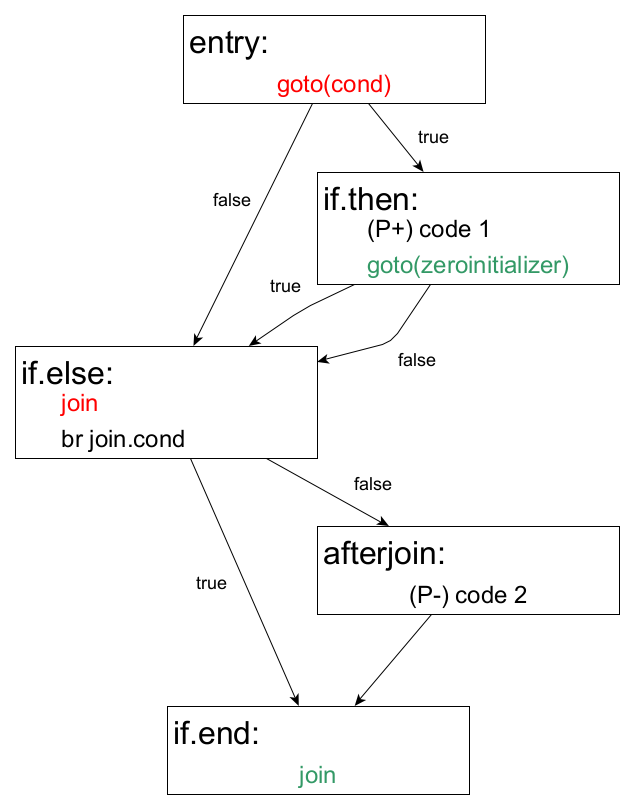
\includegraphics[scale=0.27]{Images/if-else-BE-current.png}
  \caption{\texttt{goto}-\texttt{join} cхема if-else в backend'е}
  \label{fig:if-goto-join-BE}
\end{figure}
\begin{figure}
  \centering
  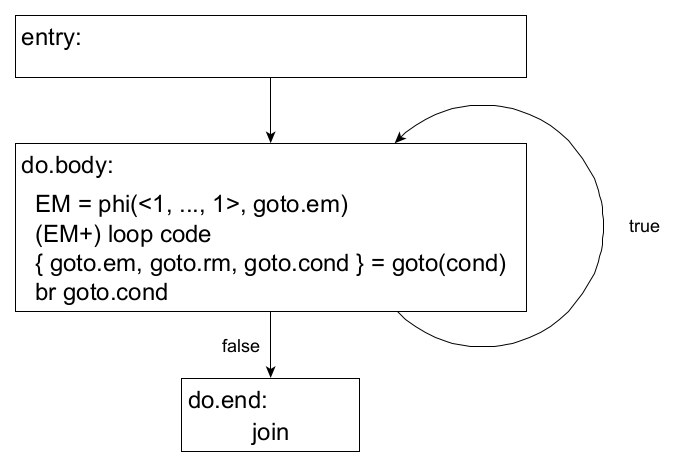
\includegraphics[scale=0.27]{Images/do-while-BE-current.png}
  \caption{\texttt{goto}-\texttt{join} cхема цикла в backend'е}
  \label{fig:loop-goto-join-BE}
\end{figure}

Для трансформирования разработанного интерфейса в уже имеющуюся модель
\texttt{goto}-\texttt{join}. Для этого надо заменить интринсик
\texttt{llvm.vector.reduce.and} или \texttt{llvm.vector.reduce.and} на
интринсик, соответствующий инструкции \texttt{goto} для вычисления условия
условного перехода, вставить соответствующий ему \texttt{join},
после чего убрать маскирование побочных эффектов.

Тогда мы получим следующие схемы для трансформации, представленные на рисунках
~\ref{fig:if-transform} и ~\ref{fig:loop-transform}.
\begin{figure}
  \centering
  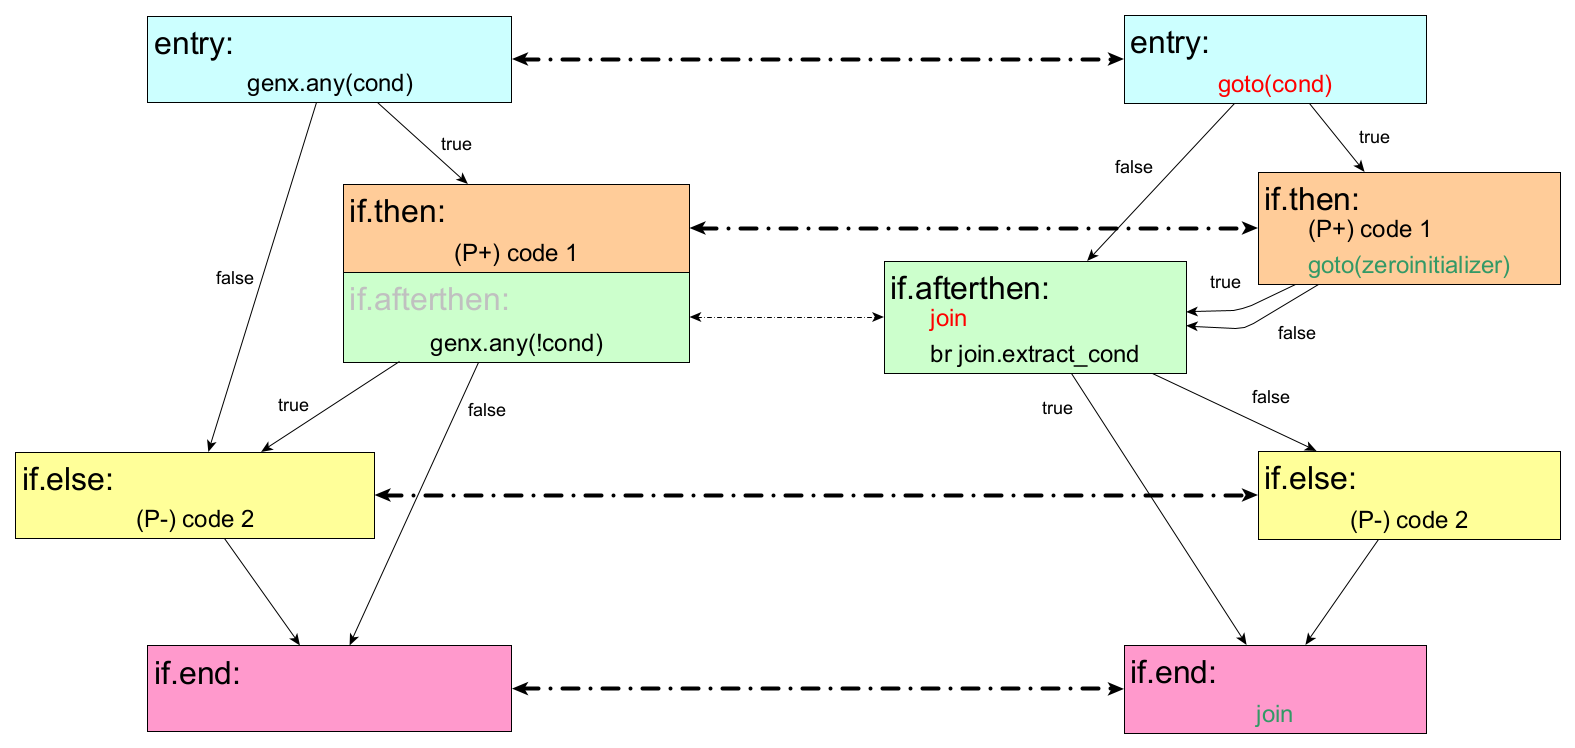
\includegraphics[width=0.5\textwidth]{Images/if-else-BE.png}
  \caption{Трансформация if-else}
  \label{fig:if-transform}
\end{figure}
\begin{figure}
  \centering
  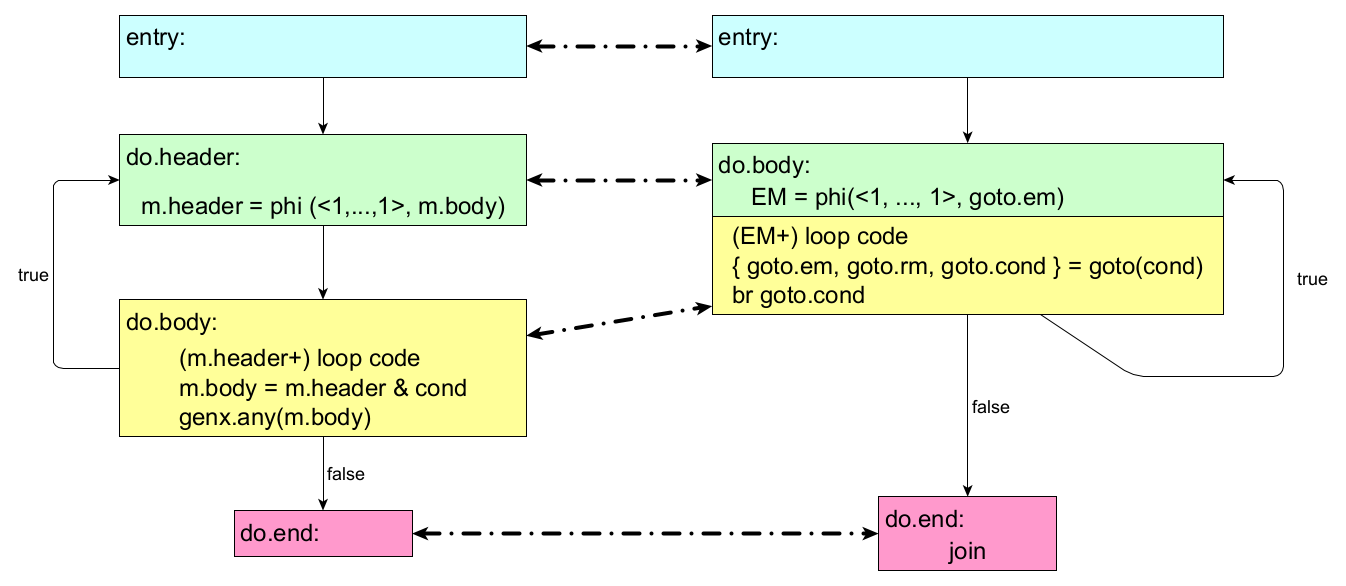
\includegraphics[width=0.5\textwidth]{Images/do-while-BE.png}
  \caption{Трансформация цикла}
  \label{fig:loop-transform}
\end{figure}
